\chapter{الرنين المغناطيسي النووي للبروتون}\label{ch:g12:proton-nmr}

في مستشفى، يستلقي مريض داخل حلقة جهاز التصوير بالرنين المغناطيسي، فتظهر على
الشاشة صورة للأنسجة الرخوة في الجسم، مبنية من أجوبة نوى الهيدروجين في مائه
ودهونه. وفي مختبر كيمياء، يُنزل أنبوب زجاجي صغير فيه بضعة مليغرامات من مركب
في تجويف مغناطيس قوي، فيظهر طيف مبني بالطريقة نفسها: مغناطيس قوي، وإشارة
راديوية، ونوى هيدروجين تجيبها. وفي مطياف الكيميائي تجيب كل \omterm{def:g9:inside-the-atom:nucleus}{نواة} هيدروجين على
نحو يختلف قليلًا بحسب جيرانها، فيكون الطيف خريطةً \omterm{def:g7:atoms-and-molecules:atom}{لذرات} الهيدروجين في
\omterm{def:g7:atoms-and-molecules:molecule}{الجزيء}.

\begin{recall}
يبيّن \omterm{def:g11:infrared:spectrum}{طيف الأشعة تحت الحمراء} الروابط التي يحويها \omterm{def:g7:atoms-and-molecules:molecule}{الجزيء}
(\cref{ch:g11:infrared}). المجموعات الوظيفية والعائلات \omterm{def:g11:organic-skeletons:isomer}{والمتماكبات}
(\cref{ch:g11:functional-groups}، \cref{ch:g11:organic-skeletons}).
\end{recall}

\begin{omfigure}
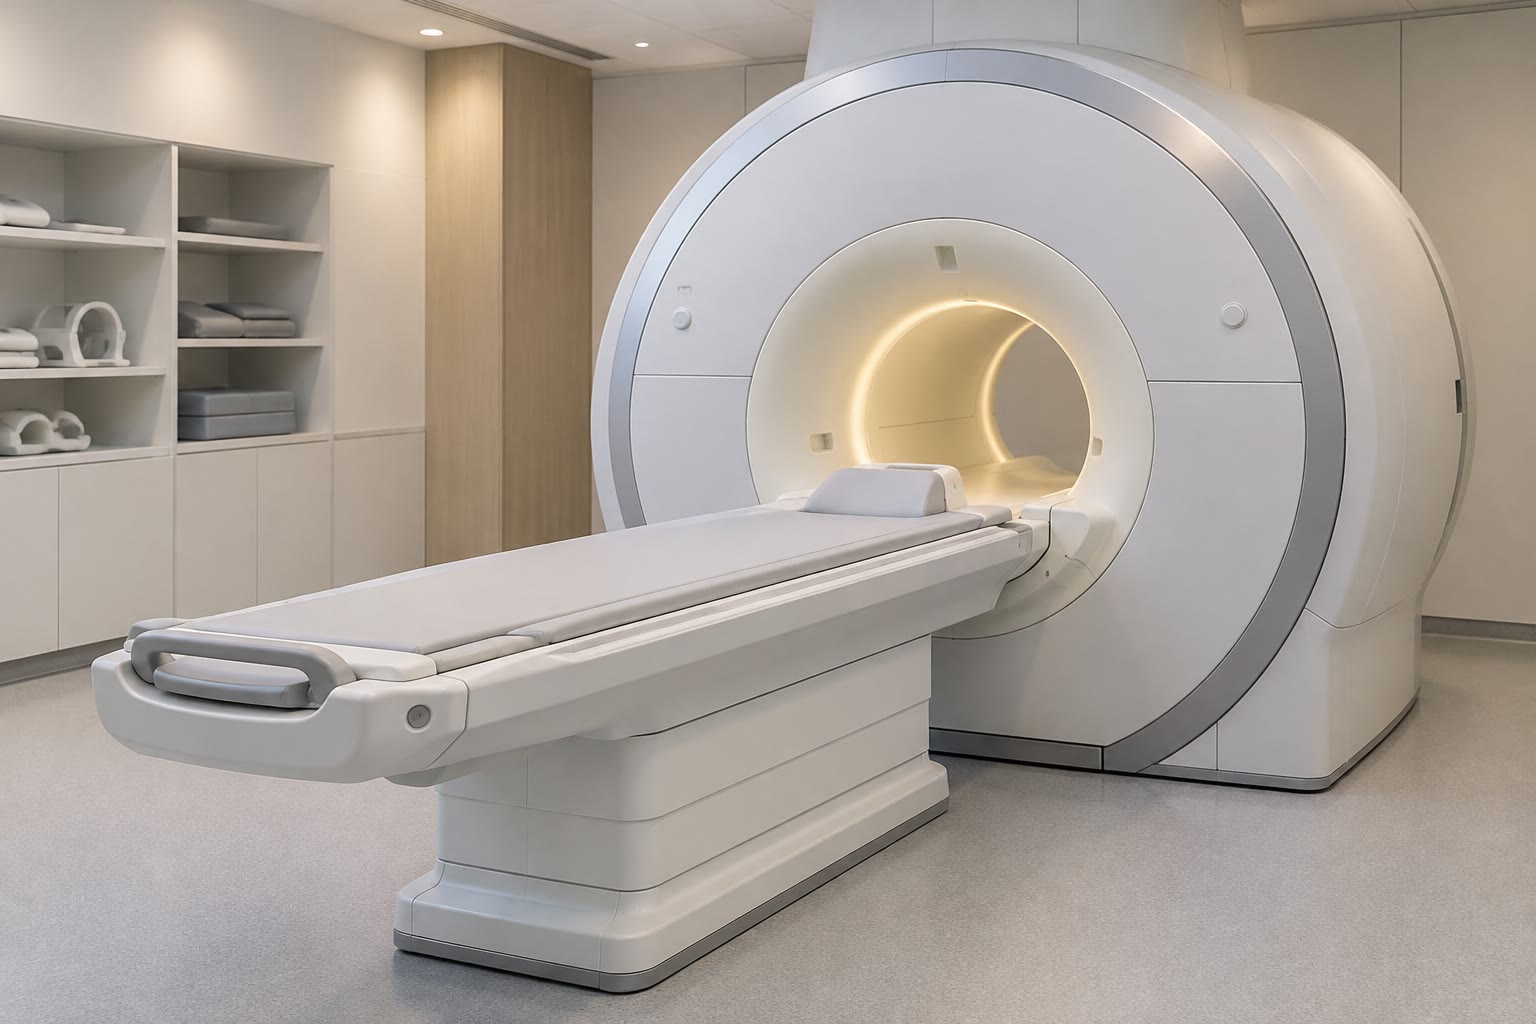
\includegraphics[width=0.48\linewidth]{images/book1/ai/g12-mri-room.jpg}

{\small جهاز تصوير بالرنين المغناطيسي: الفيزياء نفسها التي يقوم عليها مطياف
الرنين المغناطيسي النووي لدى الكيميائي.}
\end{omfigure}

\section{البروتونات في مجال مغناطيسي}

\omterm{def:g9:inside-the-atom:nucleus}{نواة} \omterm{def:g7:atoms-and-molecules:atom}{ذرة} الهيدروجين \omterm{def:g9:inside-the-atom:proton}{بروتون} واحد. فإذا وُضع في مجال مغناطيسي قوي
امتص موجات راديوية ذات تردد محدد؛ وكيفية ذلك وسببه من شأن الفيزياء، ولا
حاجة إليهما هنا. وما يهم الكيميائي هو أن \omterm{def:g9:inside-the-atom:nucleus}{الإلكترونات} المحيطة \omterm{def:g9:inside-the-atom:proton}{بالبروتون} تحجبه
قليلًا عن المجال، وأن هذا الحجب يتوقف على \omterm{def:g7:atoms-and-molecules:atom}{الذرات} القريبة: \omterm{def:g9:inside-the-atom:proton}{فالبروتون} المجاور
\omterm{def:g7:atoms-and-molecules:atom}{لذرة} أكسجين \omterm{def:g11:polarity-and-cohesion:electronegativity}{كهرسلبية}، تجذب \omterm{def:g9:inside-the-atom:nucleus}{الإلكترونات} بعيدًا عنه، يمتص عند
تردد يختلف قليلًا عن تردد \omterm{def:g9:inside-the-atom:proton}{بروتون} في سلسلة هيدروكربونية. والفروق
ضئيلة، بضعة أجزاء من المليون من التردد، وتُعطى
بالأجزاء في المليون.

\begin{omfigure}
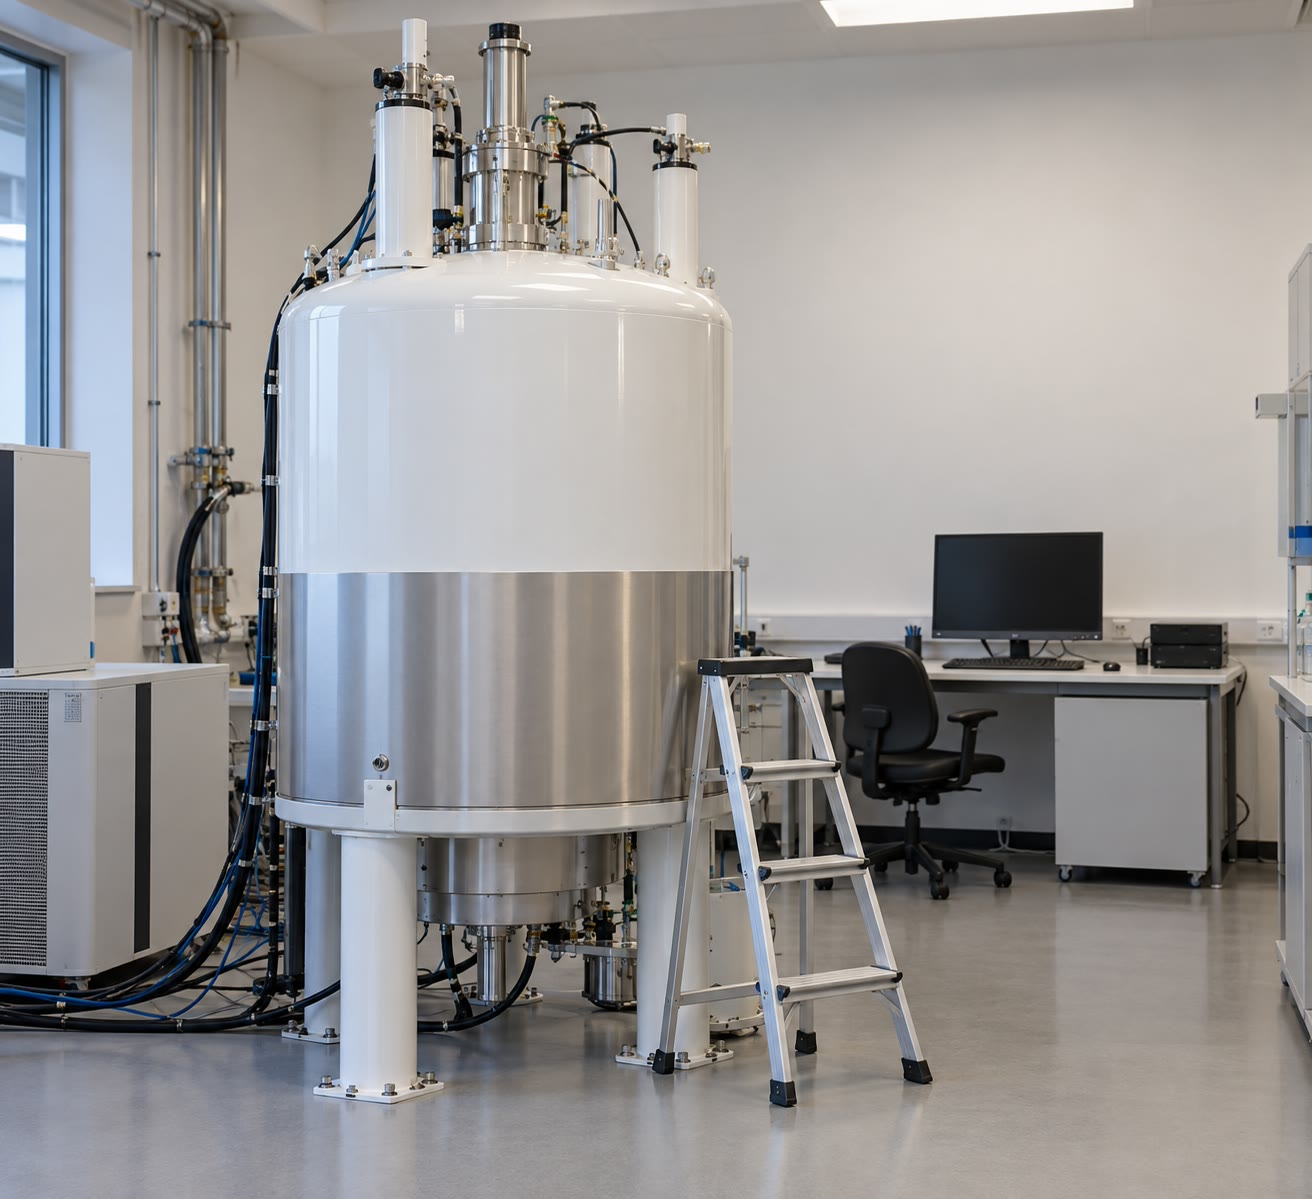
\includegraphics[width=0.42\linewidth]{images/book1/ai/g12-nmr-magnet.jpg}

{\small مغناطيس مطياف الرنين المغناطيسي النووي.}
\end{omfigure}

\begin{definition}[طيف الرنين المغناطيسي النووي، الانزياح الكيميائي]\label{def:g12:proton-nmr:spectrum}
يبيّن \emph{طيف الرنين المغناطيسي النووي}\index{طيف الرنين المغناطيسي النووي} \omterm{def:g9:inside-the-atom:proton}{للبروتون} (NMR)
الإشارات التي تمتصها نوى الهيدروجين في
مركب. وموضع الإشارة هو \emph{انزياحها
الكيميائي}\index{انزياح كيميائي} $\delta$، بالأجزاء في المليون (\si{ppm})،
مقيسًا انطلاقًا من إشارة مركب مرجعي، هو رباعي ميثيل السيلان
\ce{Si(CH3)4} (TMS)، المثبتة عند $\delta = 0$. ويُرسم محور $\delta$
متزايدًا من اليمين إلى اليسار.
\end{definition}

\begin{proposition}[الانزياح يتوقف على الجيران]\label{prop:g12:proton-nmr:shift}
% ledger: nmrr:CH3, nmrr:CH2, nmrr:allylic, nmrr:ketone, nmrr:halide, nmrr:alcohol, nmrr:vinylic, nmrr:aryl, nmrr:aldehyde, nmrr:acid
يتوقف \omterm{def:g12:proton-nmr:spectrum}{الانزياح الكيميائي} \omterm{def:g9:inside-the-atom:proton}{للبروتون} على \omterm{def:g7:atoms-and-molecules:atom}{الذرات} القريبة منه: فكلما
اقترب من \omterm{def:g7:atoms-and-molecules:atom}{ذرة} \omterm{def:g11:polarity-and-cohesion:electronegativity}{كهرسلبية} أو من \omterm{def:g10:lewis-and-shape:multiple-bond}{رابطة ثنائية} كبر
انزياحه. والمجالات النموذجية، بالوحدة \si{ppm}:
\begin{center}
\small
\begin{tabular}{ll@{\qquad}ll}
\hline
البيئة & $\delta$ & البيئة & $\delta$ \\
\hline
\ce{CH3} في سلسلة & 0.7--1.3 & \ce{H-C-O} (\omterm{def:g11:functional-groups:alcohol}{كحول}، إيثر، \omterm{def:g11:functional-groups:carboxylic-acid}{إستر}) & 3.3--4.5 \\
\ce{CH2} في سلسلة & 1.2--1.6 & \ce{H-C=C} & 4.5--6.5 \\
\ce{H-C-C=C} & 1.6--2.2 & H على حلقة بنزين & 6.5--8.0 \\
\ce{H-C-C=O} & 2.0--2.4 & \omterm{def:g11:functional-groups:carbonyl}{ألدهيد} \ce{-CHO} & 9.7--10.0 \\
\ce{H-C-X} (\omterm{def:g10:electron-shells:family}{هالوجين}) & 2.5--4.0 & حمض \ce{-COOH} & 11.0--12.0 \\
\hline
\end{tabular}
\end{center}
\end{proposition}

\begin{proof}
مقيسة على مركبات كثيرة. فالجار الكهرسلبي يجذب
\omterm{def:g9:inside-the-atom:nucleus}{الإلكترونات} بعيدًا عن \omterm{def:g9:inside-the-atom:proton}{البروتون}، فيقل حجبه ويمتص عند
انزياح أكبر.
\end{proof}

\begin{omfigure}
\begin{tikzpicture}[font=\small, x=0.75cm, y=0.5cm]
  % delta axis reversed: x = 12 - delta
  \draw[->] (0,0) -- (12.4,0) node[right] {};
  \foreach \d in {12,11,10,9,8,7,6,5,4,3,2,1,0}
    \draw ({12-\d},0) -- ({12-\d},-0.2) node[below, font=\footnotesize] {\d};
  \node[below=14pt] at (6,-0.3) {$\delta$ (\si{ppm})};
  \foreach \a/\b/\y/\c/\l in {
      11.0/12.0/1/omThm/{\ce{COOH}},
      9.7/10.0/2/omThm/{\ce{CHO}},
      6.5/8.0/1/black!60/{حلقة البنزين},
      4.5/6.5/2/omMeth/{\ce{C=C-H}},
      3.3/4.5/3/omDef/{\ce{H-C-O}},
      2.0/2.4/4/omProp/{\ce{H-C-C=O}},
      0.7/1.6/5/black!45/{\foreignlanguage{arabic}{\ce{CH3} و\ce{CH2} في السلاسل}}} {
    \fill[\c, rounded corners=1pt] ({12-\b},{\y-0.3}) rectangle ({12-\a},{\y+0.3});
    \node[anchor=west, font=\footnotesize] at ({12-\a+0.1},\y) {\l};
  }
  \draw[thick] (12,0) -- (12,0.6) node[above, font=\footnotesize] {TMS};
\end{tikzpicture}

{\small مواضع امتصاص \omterm{def:g9:inside-the-atom:proton}{البروتونات}، بحسب البيئة. \omterm{def:g9:inside-the-atom:proton}{البروتونات} القريبة من الأكسجين، أو من
\omterm{def:g10:lewis-and-shape:multiple-bond}{رابطة ثنائية} أو من مجموعة حمضية تظهر في يسار الطيف.}
\end{omfigure}

\begin{inthelab}[تحضير أنبوب الرنين المغناطيسي النووي]
تُذاب بضعة مليغرامات من المركب في نحو
\qty{0.6}{mL} من \omterm{def:g6:solutions-and-solubility:solute}{مذيب} استُبدلت \omterm{def:g7:atoms-and-molecules:atom}{بذرات} الهيدروجين فيه \omterm{def:g7:atoms-and-molecules:atom}{ذرات}
الدوتيريوم (\ce{CDCl3}، الكلوروفورم المُدَوْتَر)، فلا يعطي أي إشارة؛ ويضاف
أثر من TMS مرجعًا. ويُرشَّح \omterm{def:g2:mixing-and-dissolving:dissolve}{المحلول} في
أنبوب زجاجي رفيع، يُسد ويوسَم ويُنزل في المغناطيس.
\end{inthelab}

\section{البروتونات المتكافئة}

\begin{definition}[البروتونات المتكافئة]\label{def:g12:proton-nmr:equivalent}
تكون \omterm{def:g9:inside-the-atom:proton}{البروتونات} \emph{بروتونات متكافئة}\index{بروتونات متكافئة} إذا كانت
لها البيئة نفسها في \omterm{def:g7:atoms-and-molecules:molecule}{الجزيء}، فتمتص عند
الانزياح نفسه. وكل مجموعة من \omterm{def:g9:inside-the-atom:proton}{البروتونات} المتكافئة تعطي إشارة واحدة. \omterm{def:g9:inside-the-atom:proton}{والبروتونات}
الثلاثة لمجموعة \ce{CH3} متكافئة دائمًا.
\end{definition}

\begin{example}[عدّ المجموعات]\label{ex:g12:proton-nmr:groups}
للبروبانون، \ce{CH3-CO-CH3}، ستة \omterm{def:g9:inside-the-atom:proton}{بروتونات} لكن مجموعة واحدة: فمجموعتا
\ce{CH3} متماثلتان، واحدة في كل جانب من \ce{C=O}. وللإيثانول،
\ce{CH3-CH2-OH}، ثلاث مجموعات (\ce{CH3}، \ce{CH2}، \ce{OH})، ولإيثانوات
الإيثيل، \ce{CH3-CO-O-CH2-CH3}، ثلاث كذلك: \ce{CH3}
المجاورة لمجموعة \ce{C=O}، و\ce{CH2} المجاورة \omterm{def:g7:atoms-and-molecules:atom}{لذرة} \ce{O}، و\ce{CH3} في
الطرف.
\end{example}

\section{التكامل}

\begin{definition}[منحنى التكامل]\label{def:g12:proton-nmr:integration}
\emph{منحنى التكامل}\index{منحنى التكامل} \omterm{def:g12:proton-nmr:spectrum}{لطيف الرنين المغناطيسي النووي}
منحنى يُرسم فوق الإشارات، ويرتفع بدرجة عند كل إشارة:
وارتفاع كل درجة متناسب مع عدد \omterm{def:g9:inside-the-atom:proton}{البروتونات} التي
تعطي تلك الإشارة.
\end{definition}

\begin{example}[قراءة الدرجات]\label{ex:g12:proton-nmr:steps}
في طيف الإيثانول، تقيس الدرجات فوق الإشارات الثلاث 2 و1
و3 وحدات، من اليسار إلى اليمين: \ce{CH2} و\ce{OH} و\ce{CH3}. ولا تهم إلا
النسب: فدرجات من 12 و6 و18 mm تقول الشيء نفسه.
\end{example}

\section{التعدد وقاعدة \texorpdfstring{$n+1$}{n+1}}


\begin{definition}[المتعدد، قاعدة $n+1$]\label{def:g12:proton-nmr:multiplet}
كثيرًا ما تنقسم الإشارة إلى عدة خطوط متقاربة: فتكون \emph{متعددًا}\index{متعدد}
(أحادية، ثنائية، ثلاثية، رباعية، \dots{} لخط واحد أو 2 أو 3 أو 4 خطوط). وبحسب
\emph{قاعدة $n+1$}\index{قاعدة n+1@قاعدة $n+1$}، فإن مجموعة من \omterm{def:g12:proton-nmr:equivalent}{البروتونات المتكافئة}
تحمل \omterm{def:g7:atoms-and-molecules:atom}{ذرات} الكربون المجاورة لها $n$ بروتونًا في المجموع، غير متكافئة
معها، تعطي إشارة من $n+1$ خطًا، شداتها بنسب
مثلث باسكال.
\end{definition}

\begin{proposition}[الانقسام بالجيران]\label{prop:g12:proton-nmr:n-plus-one}
في \omterm{def:g7:atoms-and-molecules:molecule}{جزيء} \ce{CH3-CH2-X} (حيث X بلا هيدروجين)، تكون إشارة \ce{CH3}
ثلاثية (بروتونان مجاوران) وإشارة \ce{CH2} رباعية
(3 \omterm{def:g9:inside-the-atom:proton}{بروتونات} مجاورة). أما \omterm{def:g9:inside-the-atom:proton}{البروتونات} المرتبطة \omterm{def:g7:atoms-and-molecules:atom}{بذرة} أكسجين أو نيتروجين
فتعطي عادةً إشارة أحادية ولا تقسم إشارات جيرانها.
\end{proposition}

\begin{proof}
نقبله: فكل \omterm{def:g9:inside-the-atom:proton}{بروتون} مجاور يزيح الإشارة قليلًا إلى الأعلى أو إلى الأسفل
بحسب حالته هو، وتعطي التركيبات $n+1$ خطًا؛ ويشرح مجلد السنة الأولى
الفيزياء وراء ذلك. \omterm{def:g9:inside-the-atom:proton}{والبروتونات} المرتبطة \omterm{def:g7:atoms-and-molecules:atom}{بذرة} O أو N
تتبادل بسرعة بين \omterm{def:g7:atoms-and-molecules:molecule}{الجزيئات}، فيُلغى أثرها بالمتوسط.
\end{proof}

\begin{omfigure}
\begin{tikzpicture}[font=\small]
  % Pascal's triangle
  \foreach \r/\vals in {0/{1}, 1/{1,1}, 2/{1,2,1}, 3/{1,3,3,1}, 4/{1,4,6,4,1}} {
    \foreach \v [count=\i from 0] in \vals
      \node at ({\i*0.7 - \r*0.35}, {-\r*0.55}) {\v};
    \node[anchor=east, font=\footnotesize, black!60] at (-2.0,{-\r*0.55}) {$n = \r$};
  }
  % multiplets
  \begin{scope}[xshift=4.2cm, yshift=-2.4cm]
    \foreach \x/\name/\hs in {0/أحادية/{1}, 1.4/ثنائية/{1,1}, 3.0/ثلاثية/{1,2,1},
                              4.9/رباعية/{1,3,3,1}} {
      \foreach \h [count=\i from 0] in \hs {
        \draw[very thick, omDef] ({\x + \i*0.22},0) -- ({\x + \i*0.22},{\h*0.55});
      }
      \node[anchor=north, font=\footnotesize] at ({\x+0.3},-0.1) {\name};
    }
  \end{scope}
\end{tikzpicture}

{\small يعطي مثلث باسكال الشدات النسبية لخطوط إشارة عددها $n+1$
تقسمها $n$ \omterm{def:g9:inside-the-atom:proton}{بروتونات} مجاورة: 1:1، 1:2:1، 1:3:3:1.}
\end{omfigure}

\begin{omfigure}
\newcommand{\nmrpanel}[4]{% file part, title, xmax, ymax
\begin{tikzpicture}
\begin{axis}[width=\linewidth, height=4.2cm, x dir=reverse, xmin=0,
    xmax=#3, ymin=0, ymax=#4, ytick=\empty, axis y line=none,
    axis x line*=bottom, xlabel={\babelsublr{$\delta$ (\si{ppm})}},
    tick label style={font=\scriptsize}, label style={font=\scriptsize},
    title={\small #2}, title style={yshift=-3pt}]
  \addplot[omDef, thin] table[x=delta, y=I] {figdata/out/grade-12-proton-nmr-#1.dat};
  \addplot[omProp, thick] table[x=delta, y expr=0.15+\thisrow{integral}*0.11]
    {figdata/out/grade-12-proton-nmr-#1.dat};
\end{axis}
\end{tikzpicture}}
\begin{minipage}{0.49\linewidth}\nmrpanel{a}{A: الإيثانول}{5}{1.15}\end{minipage}\hfill
\begin{minipage}{0.49\linewidth}\nmrpanel{b}{B: إيثانوات الإيثيل}{5}{1.15}\end{minipage}

\begin{minipage}{0.49\linewidth}\nmrpanel{c}{C: البروبانون}{5}{1.15}\end{minipage}\hfill
\begin{minipage}{0.49\linewidth}\nmrpanel{e}{D: إيثانوات الميثيل}{5}{1.15}\end{minipage}

\begin{minipage}{\linewidth}\nmrpanel{d}{E: حمض البروبانويك}{12.5}{1.15}\end{minipage}

{\small أطياف الرنين المغناطيسي النووي \omterm{def:g9:inside-the-atom:proton}{للبروتون} (بالأزرق) مع منحنيات تكاملها
(بالبرتقالي؛ كل درجة متناسبة مع عدد \omterm{def:g9:inside-the-atom:proton}{بروتونات}
الإشارة التي تحتها). الانزياحات هي انزياحات أطياف مقيسة في \ce{CDCl3}؛
أما أشكال الخطوط والمسافات بينها فمرسومة من نموذج بسيط.}
\end{omfigure}

\begin{example}[قراءة الأطياف]\label{ex:g12:proton-nmr:reading}
% ledger: nmr:ethylethanoate-OCH2, nmr:ethylethanoate-COCH3, nmr:ethylethanoate-CH3, nmr:ethanol-CH2, nmr:ethanol-CH3, nmr:ethanol-OH, nmr:acetone, nmr:propanoic-CH2, nmr:propanoic-CH3, nmr:propanoic-OH, nmr:meoac-OCH3, nmr:meoac-COCH3
تعطي إيثانوات الإيثيل (B) إشارة رباعية لبروتونين عند \qty{4.12}{ppm}
(\ce{O-CH2}، مجاورة للأكسجين ولمجموعة \ce{CH3})، وإشارة أحادية لثلاثة \omterm{def:g9:inside-the-atom:proton}{بروتونات} عند
\qty{2.04}{ppm} (\ce{CH3-C=O}، بلا \omterm{def:g9:inside-the-atom:proton}{بروتون} مجاور) وإشارة ثلاثية لثلاثة
\omterm{def:g9:inside-the-atom:proton}{بروتونات} عند \qty{1.26}{ppm} (\ce{CH3}، مجاورة لمجموعة \ce{CH2}). ويعطي البروبانون (C)
إشارة أحادية وحيدة لستة \omterm{def:g9:inside-the-atom:proton}{بروتونات} عند \qty{2.16}{ppm}. ولحمض البروبانويك (E)
إشارة رباعية عند \qty{2.39}{ppm}، وثلاثية عند \qty{1.16}{ppm}،
وأحادية بعيدة إلى اليسار، عند \qty{11.7}{ppm}، هي بروتونه الحمضي.
\end{example}

\section{استعمال الأشعة تحت الحمراء والرنين المغناطيسي النووي معًا}


\begin{method}[التعرف على جزيء من طيفيه في الأشعة تحت الحمراء والرنين المغناطيسي النووي]\label{met:g12:proton-nmr:identify}
\begin{enumerate}
  \item انطلاقًا من \omterm{def:g11:organic-skeletons:formulas}{الصيغة الجزيئية}، اذكر \omterm{def:g11:organic-skeletons:isomer}{المتماكبات} الممكنة
        ومجموعاتها الوظيفية.
  \item الأشعة تحت الحمراء: ابحث عن حزمة \ce{C=O} نحو \qty{1700}{cm^{-1}}
        وعن حزم \ce{O-H} أو \ce{N-H}؛ واشطب \omterm{def:g11:organic-skeletons:isomer}{المتماكبات} التي
        لا تناسب.
  \item الرنين المغناطيسي النووي: عُدّ الإشارات (مجموعات \omterm{def:g12:proton-nmr:equivalent}{البروتونات المتكافئة})، واقرأ
        التكامل (عدد \omterm{def:g9:inside-the-atom:proton}{البروتونات} في كل مجموعة)، والتعدد (الجيران)
        والانزياحات (البيئات).
  \item اجمع القطع في بنية واحدة، وتحقق منها مقابل كل
        ملاحظة.
\end{enumerate}
\end{method}

\begin{example}[متماكبان \ce{C3H6O2}]\label{ex:g12:proton-nmr:isomers}
لنأخذ متماكبين: حمض البروبانويك، وصيغته \ce{CH3-CH2-COOH}، وإيثانوات الميثيل،
وصيغتها \ce{CH3-CO-O-CH3}. ففي الأشعة تحت الحمراء، لا يُظهر حزمة \ce{O-H} العريضة جدًا إلا
الحمض. وفي الرنين المغناطيسي النووي (الطيفان E وD)، يعطي الحمض إشارة ثلاثية ورباعية
وأحادية نحو \qty{11.7}{ppm}؛ ويعطي \omterm{def:g11:functional-groups:carboxylic-acid}{الإستر} إشارتين أحاديتين لثلاثة \omterm{def:g9:inside-the-atom:proton}{بروتونات}
لكل منهما، عند 3.66 (\ce{O-CH3}) و\qty{2.05}{ppm} (\ce{CH3-C=O})، إذ لا
تحمل أي \omterm{def:g7:atoms-and-molecules:atom}{ذرة} كربون في \omterm{def:g11:functional-groups:carboxylic-acid}{الإستر} \omterm{def:g9:inside-the-atom:proton}{بروتونات} مجاورة لكربون آخر يحمل \omterm{def:g9:inside-the-atom:proton}{بروتونات}.
\end{example}

\section{تمارين}

\begin{exercise}[$\star$]\label{exo:g12:proton-nmr:1}
كم مجموعة من \omterm{def:g12:proton-nmr:equivalent}{البروتونات المتكافئة}، ومن ثم كم إشارة، تعطي هذه
\omterm{def:g7:atoms-and-molecules:molecule}{الجزيئات}: الميثان؛ الإيثان \ce{CH3-CH3}؛ البروبان؛ الميثانول
\ce{CH3-OH}؛ الميثوكسي ميثان \ce{CH3-O-CH3}؟
\end{exercise}

\begin{exercise}[$\star$]\label{exo:g12:proton-nmr:2}
لمجموعة من \omterm{def:g9:inside-the-atom:proton}{البروتونات} بروتونان مجاوران على الكربون التالي. كم
خطًا لإشارتها، وبأي نسب؟ والسؤال نفسه لثلاثة جيران
ولصفر جار.
\end{exercise}

\begin{exercise}[$\star$]\label{exo:g12:proton-nmr:3}
لطيف ثلاث إشارات درجات تكاملها 15 و10
و15 mm. وللجزيء 8 \omterm{def:g9:inside-the-atom:proton}{بروتونات}. كم بروتونًا تمثل كل
إشارة؟
\end{exercise}

\begin{exercise}[$\star$]\label{exo:g12:proton-nmr:4}
مستعينًا بجدول الانزياحات، أين تتوقع إشارة \omterm{def:g9:inside-the-atom:proton}{بروتون}
مجموعة \omterm{def:g11:functional-groups:carbonyl}{ألدهيد}؟ وإشارة مجموعة \ce{CH3} في سلسلة؟
\end{exercise}

\begin{exercise}[$\star$]\label{exo:g12:proton-nmr:5}
لماذا يُختار المرجع TMS بحيث تكون بروتوناته كلها متكافئة؟
ولماذا يكون \omterm{def:g6:solutions-and-solubility:solute}{المذيب} مُدَوْتَرًا؟
\end{exercise}

\begin{exercise}[$\star\star$]\label{exo:g12:proton-nmr:6}
تنبأ بطيف الكلورو إيثان \ce{CH3-CH2-Cl}: عدد الإشارات،
والتكامل، والتعدد، والانزياحات التقريبية.
\end{exercise}

\begin{exercise}[$\star\star$]\label{exo:g12:proton-nmr:7}
تنبأ بطيف بروبان-2-ول، \ce{(CH3)2CH-OH}: ولا سيما
تعدد إشارة \ce{CH3} وإشارة \ce{CH} (افترض أن
\ce{OH} تعطي إشارة أحادية ولا تقسم غيرها).
\end{exercise}

\begin{exercise}[$\star\star$]\label{exo:g12:proton-nmr:8}
ثلاثة أطياف: (a) إشارة أحادية واحدة؛ (b) رباعية وأحادية وثلاثية،
تكاملاتها 2:3:3؛ (c) رباعية وثلاثية وأحادية بعيدة إلى اليسار،
تكاملاتها 2:3:1. طابق بينها وبين إيثانوات الإيثيل والبروبانون
وحمض البروبانويك.
\end{exercise}

\begin{exercise}[$\star\star$]\label{exo:g12:proton-nmr:9}
مستعينًا بمخطط الانزياحات، اشرح لماذا تقع إشارة \ce{CH2} في إيثانوات الإيثيل
(\qty{4.12}{ppm}) بعيدًا إلى يسار إشارة \ce{CH3} في مجموعة الإيثيل
نفسها (\qty{1.26}{ppm}).
\end{exercise}

\begin{exercise}[$\star\star$]\label{exo:g12:proton-nmr:10}
يُظهر مركب \ce{C3H6O} حزمة قوية في الأشعة تحت الحمراء عند
\qty{1715}{cm^{-1}} وإشارة أحادية واحدة في الرنين المغناطيسي النووي. تعرّف عليه. ولماذا
يُستبعد البروبانال؟
\end{exercise}

\begin{exercise}[$\star\star$]\label{exo:g12:proton-nmr:11}
في طيف الإيثانول، لماذا تكون إشارة \ce{OH} أحادية، ولماذا
تظهر \ce{CH2} رباعيةً لا إشارةً
أعقد؟
\end{exercise}

\begin{exercise}[$\star\star\star$]\label{exo:g12:proton-nmr:12}
أعطِ بنى أربعة \omterm{def:g11:organic-skeletons:isomer}{متماكبات} \ce{C4H8O2} هي \omterm{def:g11:functional-groups:carboxylic-acid}{إسترات} أو أحماض
(حمض البوتانويك، إيثانوات الإيثيل، بروبانوات الميثيل، ميثانوات البروبيل،
\dots) وتنبأ، لكل منها، بعدد إشارات الرنين المغناطيسي النووي
وتعددها.
\end{exercise}

\begin{exercise}[$\star\star\star$]\label{exo:g12:proton-nmr:13}
تُرَجّ قطرة من الماء الثقيل \ce{D2O} مع \omterm{def:g2:mixing-and-dissolving:dissolve}{محلول} من الإيثانول، ثم
يُسجَّل الطيف من جديد: فتختفي إشارة. أي إشارة هي، ولماذا؟
وكيف يساعد ذلك على التعرف على \omterm{def:g9:inside-the-atom:proton}{بروتونات} \ce{O-H}؟
\end{exercise}

\begin{exercise}[$\star\star\star$]\label{exo:g12:proton-nmr:14}
تحوي عيّنة من إيثانوات الإيثيل بعض الإيثانول. أي إشارات إضافية
تظهر في الطيف؟ وإذا كان تكامل الإشارة الأحادية عند
\qty{2.04}{ppm} يساوي 30 mm وتكامل إشارة ثلاثية إضافية صغيرة عند
\qty{1.23}{ppm} يساوي 3 mm، فقدّر النسبة بين كميتي الإيثانول
\omterm{def:g11:functional-groups:carboxylic-acid}{والإستر}.
\end{exercise}

\begin{exercise}[$\star\star\star$]\label{exo:g12:proton-nmr:15}
صيغة 2-ميثيل بروبان-1-ول هي \ce{(CH3)2CH-CH2-OH}. تنبأ بطيفه:
الإشارات، وتكاملاتها، وتعدد إشارتي \ce{CH3}
و\ce{CH2}. وأي إشارة لها أكبر عدد من الخطوط؟
\end{exercise}

\section{مسألة: المذيب المجهول}

\begin{problem}[{مسألة نهاية الأسبوع --- قارورة \omterm{def:g6:solutions-and-solubility:solute}{مذيب} لا يحمل لصاقها إلا
\ce{C4H8O2}: ما هو، وما ارتفاع كل درجة من منحنى
تكامله؟}]
\label{pb:g12:proton-nmr:1}
% ledger: nmr:ethylethanoate-OCH2, nmr:ethylethanoate-COCH3, nmr:ethylethanoate-CH3, ir:CO-ester, ir:OH-acid
قارورة \omterm{def:g6:solutions-and-solubility:solute}{مذيب} في مخزن لا يحمل لصاقها إلا «\ce{C4H8O2}». ويُظهر
طيفها في الأشعة تحت الحمراء حزمة قوية عند \qty{1740}{cm^{-1}} ولا حزمة
فوق \qty{3100}{cm^{-1}}. ويُظهر طيفها في الرنين المغناطيسي النووي ثلاث إشارات: إشارة
رباعية عند \qty{4.12}{ppm}، وأحادية عند \qty{2.04}{ppm} وثلاثية عند
\qty{1.26}{ppm}. ويرتفع \omterm{def:g12:proton-nmr:integration}{منحنى التكامل} بما مجموعه \qty{72}{mm}.

\medskip
\noindent\textbf{الجزء الأول --- المرشحات.}
\begin{enumerate}
  \item تحقق من أن \ce{C4H8O2} تناسب إسترًا أو حمضًا كربوكسيليًا ليس في
        سلسلته إلا روابط أحادية.
  \item أعطِ الصيغ نصف البنيوية وأسماء حمض البوتانويك
        \omterm{def:g11:functional-groups:carboxylic-acid}{والإسترات} الثلاثة إيثانوات الإيثيل وبروبانوات الميثيل وميثانوات
        البروبيل.
  \item أي \omterm{def:g11:functional-groups:functional-group}{مجموعة وظيفية} تشترك فيها مثنى مثنى؟
\end{enumerate}

\medskip
\noindent\textbf{الجزء الثاني --- الأشعة تحت الحمراء.}
\begin{enumerate}[resume]
  \item ماذا تكشف الحزمة عند \qty{1740}{cm^{-1}}؟
  \item ماذا كان سيُظهر حمض البوتانويك مما هو غائب هنا؟ واشطبه
        من القائمة.
  \item أتستطيع الأشعة تحت الحمراء وحدها أن تختار بين \omterm{def:g11:functional-groups:carboxylic-acid}{الإسترات} الثلاثة؟
\end{enumerate}

\medskip
\noindent\textbf{الجزء الثالث --- الرنين المغناطيسي النووي.}
\begin{enumerate}[resume]
  \item كم مجموعة من \omterm{def:g12:proton-nmr:equivalent}{البروتونات المتكافئة} للمجهول؟
  \item ماذا توحي به الإشارتان الرباعية والثلاثية معًا؟
  \item ماذا تقول الإشارة الأحادية عن جيران بروتوناتها؟
  \item لماذا تقع الإشارة الرباعية عند انزياح كبير؟
  \item تنبأ بطيف بروبانوات الميثيل \ce{CH3-CH2-CO-O-CH3}
        (الإشارات، والتعدد، والانزياحات التقريبية). أهو المجهول؟
  \item تنبأ بطيف ميثانوات البروبيل. أهو المجهول؟
\end{enumerate}

\medskip
\noindent\textbf{الجزء الرابع --- التعرف والتكامل.}
\begin{enumerate}[resume]
  \item تعرّف على المجهول وارسم بنيته، مبيّنًا عليها كل
        إشارة.
  \item كم بروتونًا تمثل كل إشارة؟
  \item التكامل الكلي \qty{72}{mm} لثمانية \omterm{def:g9:inside-the-atom:proton}{بروتونات}. فكم
        مليمترًا لكل \omterm{def:g9:inside-the-atom:proton}{بروتون}؟
  \item احسب ارتفاع درجة الإشارة الأحادية ودرجة الإشارة الثلاثية.
  \item تحقق من أن مجموع الدرجات الثلاث \qty{72}{mm}.
  \item لإيثانوات الإيثيل رائحة حلوى الإجاص: أيتفق ذلك مع
        العائلة التي وجدتها؟
  \item اذكر الجواب النهائي: ما ارتفاع درجة تكامل
        الإشارة الرباعية؟
\end{enumerate}
\end{problem}
